\documentclass[border=14pt,tikz]{standalone}
\usepackage{fontspec}
\setmainfont{Helvetica Neue}
\setsansfont{Helvetica Neue}
\setmonofont{Menlo}
\usepackage{amsmath}
\usepackage{tikz}
\usetikzlibrary{positioning, arrows.meta, shapes.geometric}

\definecolor{kernel}{HTML}{E3F2FD}
\definecolor{kernelborder}{HTML}{2196F3}
\definecolor{state}{HTML}{E8F5E9}
\definecolor{stateborder}{HTML}{4CAF50}
\definecolor{choice}{HTML}{FFF3E0}
\definecolor{choiceborder}{HTML}{FF9800}

\begin{document}
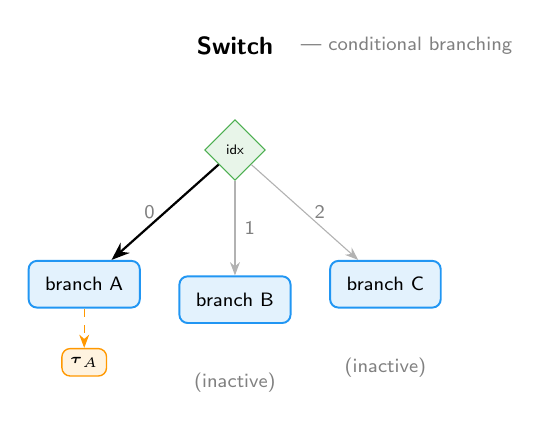
\begin{tikzpicture}[
    >=Stealth,
    node distance=1cm and 1.2cm,
    kern/.style={draw, rounded corners=3pt, inner sep=6pt,
                 font=\sffamily\scriptsize, fill=kernel, draw=kernelborder, line width=0.7pt},
    ch/.style={draw, rounded corners=3pt, inner sep=3pt,
               font=\ttfamily\tiny, fill=choice, draw=choiceborder, line width=0.5pt},
    title/.style={font=\sffamily\small\bfseries},
    annot/.style={font=\sffamily\scriptsize, text=black!50},
]

\node[title] (swt) {Switch};
\node[annot, right=3pt of swt] {--- conditional branching};

\node[draw, diamond, inner sep=3pt, fill=state, draw=stateborder,
      font=\sffamily\tiny, below=0.7cm of swt] (idx) {idx};

\node[kern, below left=1.2cm and 1cm of idx] (b0) {branch A};
\node[kern, below=1.2cm of idx] (b1) {branch B};
\node[kern, below right=1.2cm and 1cm of idx] (b2) {branch C};

\draw[->, line width=0.8pt] (idx) -- (b0) node[midway, left, annot] {0};
\draw[->, line width=0.4pt, black!30] (idx) -- (b1) node[midway, right, annot] {1};
\draw[->, line width=0.4pt, black!30] (idx) -- (b2) node[midway, right, annot] {2};

\node[ch, below=0.5cm of b0] (swc) {$\boldsymbol{\tau}_A$};
\draw[->, dashed, choiceborder] (b0) -- (swc);

\node[annot, below=0.5cm of b1] {(inactive)};
\node[annot, below=0.5cm of b2] {(inactive)};

\end{tikzpicture}
\end{document}
